\chapter{Overenie riešenia}

Keďže sme natrénovali viacero modelov, a metóda RISEI má veľké množstvo parametrov zvolili sme nasledovnú stratégiu pri overovaní riešenia, tak aby sme nemuseli overovať všetky možné kombinácie parametrov/architektúr a dokázali vykonať všetky navrhnuté experimenty (Sekcia \ref{sec:design_experiments}) v stanovenom čase.

\begin{enumerate}
    \item Výber architektúry neurónovej siete na ktorej budeme overovať metódu RISEI a porovnávať ju z ostatnými. \textit{Ktorý z natrénovaných modelov je najvhodnejší pre navrhnutú metódu?}
    \item Overenie metódy RISEI. \textit{Dávajú výsledky z navrhnutej metódy zmysel a nie sú náhodné?}: 
         \begin{itemize}
             \item Overenie stability tepelných máp.
             \item Overenie kvality tepelných máp (metriky \textit{insertion} a \textit{deletion}).
         \end{itemize}
    \item Porovnanie kvality tepelných máp s metódou RISE (s doimplementovanou podporou pre 3D snímky) - \textit{je navrhnutá metóda lepšia ako metóda, z ktorej vychádza?}
    \item Overenie správnosti tepelných máp a porovnanie s inými metódami - GradCAM, Guided Backprop, Guided GradCAM. \textit{Sú tepelné mapy nie len kvalitné, ale dávajú zmysel v kontexte anatómie mozgu? Ako sú na tom iné metódy?}
\end{enumerate}

\paragraph{Adresovanie náhodnosti metódy RISE pri porovnávaní dvoch roznych modelov}

Keďže vygenerované masky sú náhodné, pri porovnávaní dvoch metód (kombinácii rôznych parametrov metódy RISEI) generujeme rovnaké binárne masky pre každý i-ty snímok, tj. zakryté pozície sú rovnaké, rôzna je len hodnota zakrytia. Vygenerované binárne masky pre jednotlivé snímky v testovacej sade sú stále náhodné (a teda aj medzi sebou rôzne). Rovnaké sú len binárne masky pre dve rôzne generovania masiek pre ten istý snímok v testovacej sade. Takto dosiahneme presnejšie výsledky, pretože nebudeme porovnávať miesto prekrytia ale spôsob - hodnotu prekrytia.

\section{Experimenty}

\subsection{Výber architektúry neurónovej siete pre ďaľšie experimenty \label{sec:experiment_rise_various_architectures}}

V tomto experiemnte sme porovnali metódu RISE na nami natrénovaných modeloch s cieľom vybrať jeden z nich pre ďaľšie experimenty (keďže experimenty sú časovo náročné, nechceme ich robiť na všetkých modeloch). Vybrali sme najlepšie natrénované modely pre každú architektúru (Tabuľka \ref{tab:model_training_results}). Použili sme nami implementovanú metódu RISEI pričom sme nastavili jej parametre tak, aby fungovala ako metóda RISE.
Parametre sme nastavili nasledovne: $s = 8$, $p = 1/3$, $b1 = 0$, $b2 = 1$ (opis parametrov sa nachádza v tabuľke \ref{tab:risei_params}). Na vytvorenie tepelnej mapy sme vygenerovali 1024 masiek. Pri vyhodnocovaní metrík insertion a deletion sme nastavili veľkosť kroku na 2500 voxelov (takto trvalo vyhodnotenie tepelnej mapy ~3 minúty). Vybrali sme 25 náhodných snímiek z testovacej sady (13 AD, 12 CN), generovanie a vyhodnotenie tepelných máp k nim trvalo približne ~1 hodinu. 

Najlepšie výsledky sme dosiahli na architektúre 3D CNN (Tabuľka \ref{tab:experiment_rise_various_architectures}). Je dôležité si ale uvedomiť, že na vyhodnotenie metrík \textit{insertion} a \textit{deletion} z vytvorenej tepelnej masky sa používa model samotný - zo snímky sú pridávané/odoberané voxely pričom sa sleduje sa zmena predikcie modelu. Môže nastať teda situácia, že dva rôzne modely vytvoria dve identické tepelné mapy, pričom výsledná hodnota metriky bude rozdielna. Na základe týchto metrík teda nemôžeme tvrdiť, že jeden model vytvára lepšie tepelné mapy ako druhý. Metrika \textit{insertion} a \textit{deletion} nie je vhodná na takéto porovnanie dvoch rôznych modelov medzi sebou.
Dobrým signálom by bolo ak by hodnota metriky \textit{insertion} bola väčšia ako metriky \textit{deletion}, takto to nie je ani u jedného z modelov (najbližšie má k tomu 3D CNN). Aj kvôli tomuto sme vybrali do ďaľších experimentov model 3D CNN, zároveň na základe jeho špecificity a senzitivity môžeme tvrdiť, že nepreferuje ani jednu z tried - čo u iných modeloch tak nie je (tie preferujú AD pozorovania). Taktiež je tento model jednoduchší.

\begin{table}[]
    \centering
    \begin{tabular}{cl|r|r|r|}
        \cline{3-5}
        \multicolumn{1}{l}{} &  & \multicolumn{1}{c|}{3D CNN} & \multicolumn{1}{c|}{3D ResNET} & \multicolumn{1}{c|}{2D ResNET} \\ \hline
        \multicolumn{1}{|c|}{\multirow{2}{*}{Insertion (AUC)}} & priemer & \textbf{0.50} & 0.46 & 0.38 \\ \cline{2-2}
        \multicolumn{1}{|c|}{}                                 & medián  & \textbf{0.53} & 0.13 & 0.30 \\ \cline{1-2}
        \multicolumn{1}{|c|}{\multirow{2}{*}{Deletion (AUC)}}  & priemer & \textbf{0.53} & 0.81 & 0.62 \\ \cline{2-2}
        \multicolumn{1}{|c|}{}                                 & medián  & 0.60 & 0.83 & \textbf{0.43} \\ \hline
    \end{tabular}
    \caption{\textbf{Porovnanie metódy RISE na rôznych architektúrach.} Vybrali sme najlepšie natrénované modely pre každú architektúru (Tabuľka \ref{tab:model_training_results}). Pre insertion sú lepšie vyššie hodnoty (očakávame, že keď vložíme najpodstatnejšie voxely aktivácia bude stúpať), pre deletion sú lepšie nižšie hodnoty (očakávame, že keď ostránime najdôležitejšie voxely, aktivácia bude klesať).}
    \label{tab:experiment_rise_various_architectures}
\end{table}

\subsection{Overenie metódy RISEI}

\subsubsection{Stabilita tepelných máp \label{sec:risei_stability}}

Keďže metóda RISEI (aj metóda RISE z ktorej vychádzame) používa na generovanie tepelným máp náhodné masky, výsledná tepelná mapa je touto náhodnosťou ovplyvnená a je teda do určitej miery náhodná. Očakávame, že čím viac masiek vygenerujeme, tým bude vplyv náhodny na výslednú tepelnú mapu nižší. Keď teda pre tú istú snímku vygenerujeme niekoľko tepelných máp, tieto tepelné mapy sa budú líšiť ćo najmenej = budú stabilné.

Metóde RISEI sme nastavili nasledovné parametre $s = 8$, $p = 1/3$, $b1 = 0$, $b2 = 1$ a $b2\_value = 1$ - nepoužívame dokreslenie, keďže je časovo náročné a vykonávame veľké množštvo experimentov. Uvažujeme, že nezáleží na tom, čo je hodnota zakrytia vo vygenerovaných maskách, pokiaľ tá hodnota nie je náhodná.

Použili sme model 3D CNN so senzitivitou - 0.81 a špecificitou - 0.74.

\paragraph{Porovnanie vytvorených tepelných máp}

$N$ vytvorených tepelných máp porovnávame tak, že počítame štanardnú odchílku pre každý voxel medzi vytvorenými tepelnými mapami. Tak z tepelných máp o rozmere $[N, z, y, x]$ vznikne 3D matica štandardných odchílok $[z, y, x]$. Ak má voxel rovnakú/blízku hodnotu tepla medzi tepelnými mapammi, štandardná odchýlka nula/blízka nule. Z 3D matice štandradných odchílok vypočítame priemernú/strednú hodnotu - táto hodnota reprezentuje vzniknutú chybu medzi tepelnými mapami plynúcu z náhodnosti tepelných masiek.

\subsubsection{Experiment 1 (jedna snímka) \label{sec:risei_stability_1}}

Pre náhodný snímok vytvoríme $K$ tepelných máp, pričom tepelné mapy vytvárame z 16, 128, 256, 512, 1024, 2048, 3072, 4096, 6144, 8192, 16384 alebo 32768 masiek. Kvôli vysokej pamäťovej náročnosti, v experiementoch, v ktorých vytvárame tepelné mapy z vysokého počtu masiek vytvoríme menej tepelných máp (Tabuľka \ref{tab:risei_stability_1}). Zistili sme, že s vyšším počtom vygenerovaných masiek chyba klesá logaritmicky (Obr. \ref{fig:risei_stability_1}). Zároveň, chyba sa javí byť náhodná a nie systematická (Obrázok \ref{fig:risei_stability_error_visialisation}).

\begin{table}[]
    \centering
    \begin{tabular}{|r|r|r|}
    \hline
    \multicolumn{1}{|c|}{\begin{tabular}[c]{@{}c@{}}Počet vygenerovaných\\ masiek\end{tabular}} &
      \multicolumn{1}{c|}{\begin{tabular}[c]{@{}c@{}}Počet vytvorených\\ tepelných máp\end{tabular}} &
      \multicolumn{1}{c|}{\begin{tabular}[c]{@{}c@{}}Medián štandardnej\\ odchýlky pre voxel\\ (chyba)\end{tabular}} \\ \hline
    16    & 100 & 0.0640 \\ \hline
    128   & 100 & 0.0225 \\ \hline
    256   & 100 & 0.0160 \\ \hline
    512   & 100 & 0.0113 \\ \hline
    1024  & 100 & 0.0080 \\ \hline
    2048  & 100 & 0.0057 \\ \hline
    3072  & 50  & 0.0045 \\ \hline
    4096  & 50  & 0.0039 \\ \hline
    6144  & 25  & 0.0031 \\ \hline
    8192  & 25  & 0.0027 \\ \hline
    16384 & 15  & 0.0019 \\ \hline
    32768 & 5   & 0.0011 \\ \hline
    \end{tabular}
    \caption{Stabilita vytvorených tepelných máp podľa počtu vygenerovaných masiek pre jeden snímok. S vyšším počtom vygenerovaných máp chyba výrazne klesá. Už pri 2048 maskách je chyba zanedbateľná, keďže hodnoty voxelov v tepelných mapách sú z intervalu $<0, 1>$.}
    \label{tab:risei_stability_1}
\end{table}

\begin{figure}[h!]
    \centering
    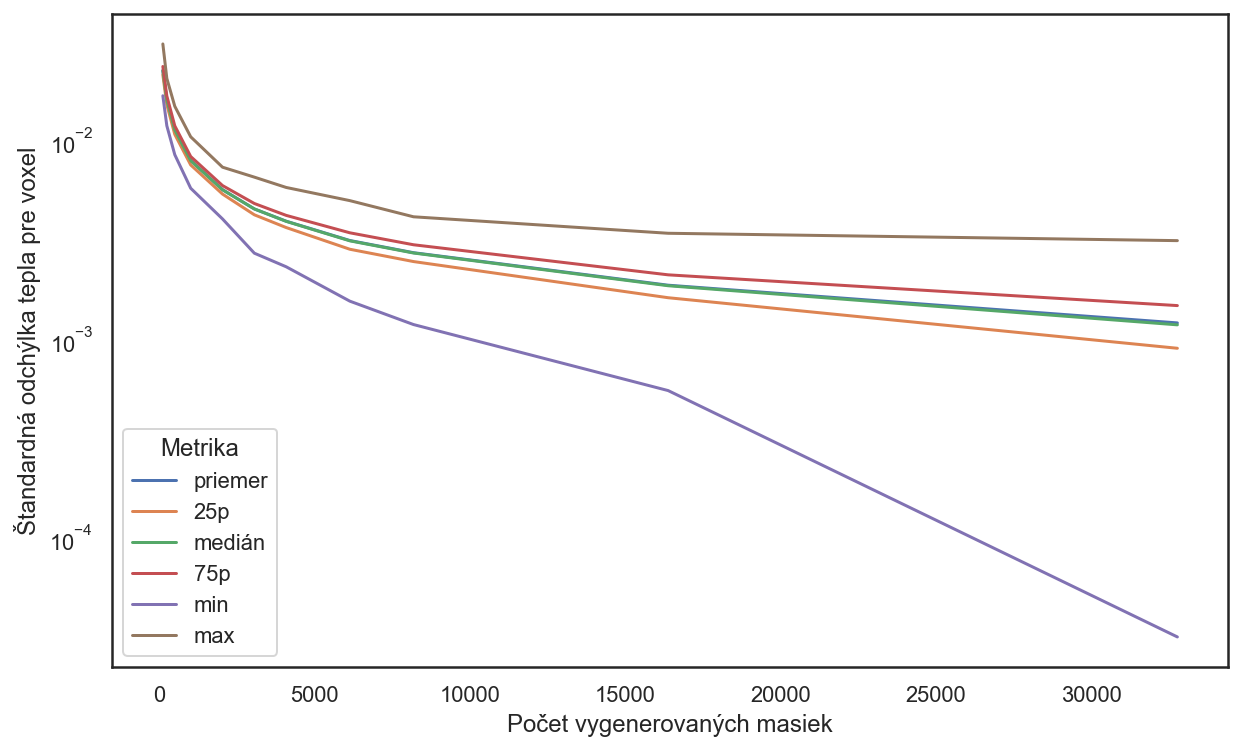
\includegraphics[width=14cm]{assets/images/risei_stability_1.png}
    \caption{Stabilita vytvorených tepelných máp podľa počtu vygenerovaných masiek. Os $y$ je v logaritmickej škále a reprezentuje chybu. Táto chyba klesá logaritmicky s vyšším počtom vygenerovaných masiek. Priemer sa veľmi blíži mediánu, preto ho na diagrame nie je takmer vôbec vidieť.}
    \label{fig:risei_stability_1}
\end{figure}

\begin{figure}[h!]
    \centering
    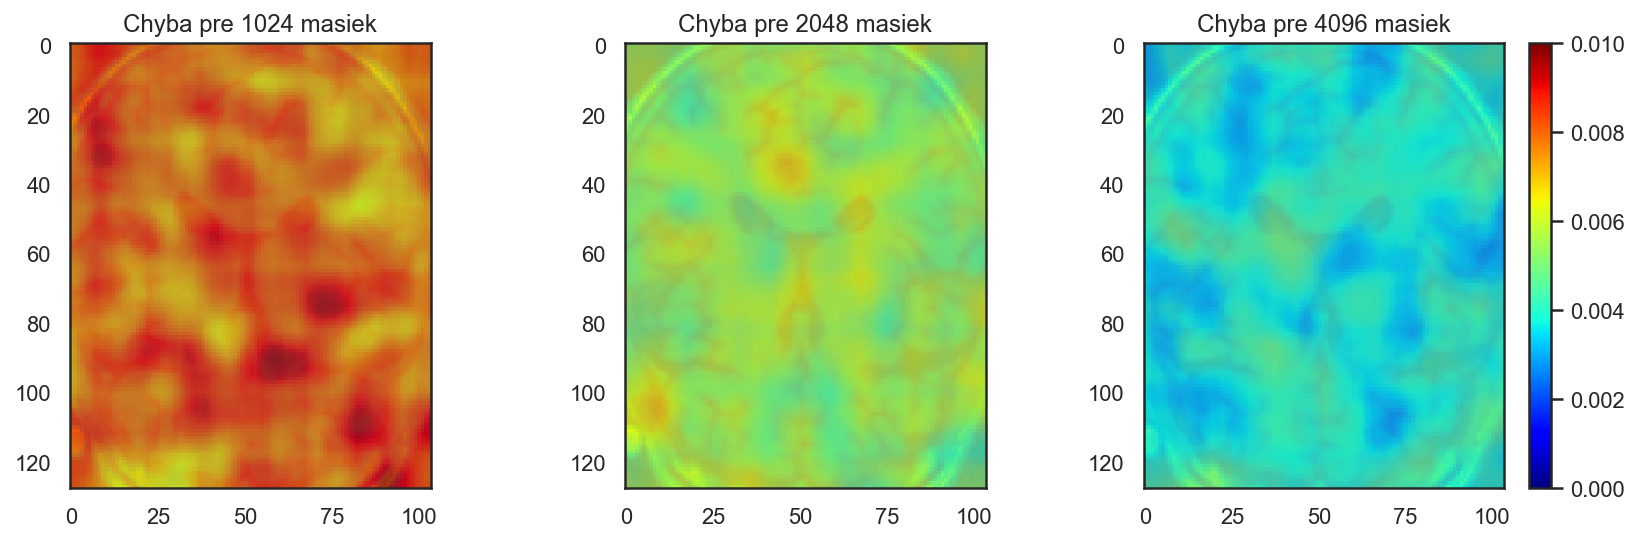
\includegraphics[width=14cm]{assets/images/risei_stability_error_visialisation.png}
    \caption{Vizualizácia chyby z generovania 1024, 2048 a 4096. Z vizualizácie je zdrejmé, že chyba je skôr náhodná ako systematická, keďže sa nachádza na rôznych častiach medzi snímkami. Škála tepla má výrazne znížené maximum oproti maximálnej možnej chybe (1) aby boli rozdiely viditeľné.}
    \label{fig:risei_stability_error_visialisation}
\end{figure}

\subsubsection{Experiment 2 (viacero snímok)}

Keďže sme v predchádzajúcom experimente overovali stabilitu iba na jednej snímke, v tomto experimente overíme stabilitu na viacero snímkach. Z testovacej sady sme vybrali 5 TP (viď. \nameref{sec:dictionary}), 5 TN, 5 FP a 5 FN pozorovaní (tj. celkovo 20 pozorovaní), podľa toho ako ich neurónová sieť označila. Takto zabezpečíme vyváženosť tried pozorovaní v experimente. Kvôli časovej aj pamäťovej náročnosti tohto experimentu sme vytvárali 10 tepelných máp pre každé jedno pozorovanie. Výsledky boli takmer identické s predchádzajúcim experimentom (Sekcia \ref{sec:risei_stability_1}) a trend poklesu chyby pri zvyšujúcom počte masiek bol zachovaný (\ref{tab:risei_stability_2}). Z oboch experimentov vyplýva, že je vhodné použiť vyšší počet masiek pri vytváraní tepelných máp, aby sa odstránil vyplyv náhody. Ako vhodným počet považujem 2048 masiek, pri tomto počte je chyba vzhľadom na hodnoty v tejeplnej mape minimálna (Tabuľka \ref{tab:risei_stability_1}, \ref{tab:risei_stability_2}).

\begin{table}[]
    \centering
    \begin{tabular}{|r|r|}
    \hline
    \multicolumn{1}{|c|}{\begin{tabular}[c]{@{}c@{}}Počet vygenerovaných\\ masiek\end{tabular}} &
      \multicolumn{1}{c|}{\begin{tabular}[c]{@{}c@{}}Medián štandardnej\\ odchýlky pre voxel\end{tabular}} \\ \hline
    16   & 0.0594 \\ \hline
    128  & 0.0207 \\ \hline
    256  & 0.0160 \\ \hline
    512  & 0.0105 \\ \hline
    1024 & 0.0074 \\ \hline
    2048 & 0.0052 \\ \hline
    3072 & 0.0043 \\ \hline
    4096 & 0.0037 \\ \hline
    \end{tabular}
    \caption{Stabilita vytvorených tepelných máp podľa počtu vygenerovaných masiek pre 20 snímiek. Trend poklesu chyby, rovnako ako v prvom experimente, (Tabuľka \ref{tab:risei_stability_1}) ostal zachovaný.}
    \label{tab:risei_stability_2}
\end{table}

Na stabilitu masiek môže mať vplyv aj parameter $p$, v tomto experimente sme použili konštantnú hodnotu $p = 1/3$. Jeho zmena môže stabilitu zvýšiť už pri menšom/až pri väčšom počte generovaných masiek. Vplyv parametra $p$ na stabilitu tepelných máp podľa počtu masiek je vhodným predmetom ďaľšieho skúmania.

\subsection{RISE vs RISEI (s rôznymi parametrami)}

V tomto experimente sme porovnali RISE a rôzne nastavenia metódy RISEI. Použili sme model 3D CNN so senzitivitou 73\% a špecificitou 71\%.

Použili sme rovnaké nastavenie parametrov, a rovnaký počet pozorovaní ako pri výbere architektúry neurónovej siete (Sekcia \ref{sec:experiment_rise_various_architectures}) a menili sme len parametre \textit{b1}, \textit{b2} a \textit{b2\_value}. Parametre \textit{in\_paint\_radius} sme nastavili na hodnotu $5$. 

Vyhodnocovali sme len metriku \textit{insertion} (aby sme čo najrýchlejšie získali prvotné výsledky), najlepšie výsledky sme dosiahlli bez použitia dokreslenia ale s prekrytím hodnotou jedna (Tabuľka \ref{tab:experiment_risei_various_configuration}). To si vysvetľujeme tým, že hodnota voxelov blízka jednej je v trénovacej sade veľmi ojedinelá (Obr. \ref{fig:test_dataset_voxel_distribution}) a neurónová sieť na základe nich nerozhoduje, takéto voxely neurónovú sieť nepomýlia. Naopak, voxely s hodnotou/blízke hodnote nula sú pomerne časté, ak na základe nich neurónová sieť rozhoduje, može to byť dôvod prečo prekrytie zaznamenalo horšie výsledky.

Metóda s dokreslením si počínala horšie ako prekrytie hodnotou jedna, ale stále lepšie ako prekrytie s hodnotou nula pôvodná metóda RISE). Zároveň dosiahla takmer identický výsledok ako prykritie mediánom hodnôt voxelov snímky.

Obrázok \ref{fig:heatmap_and_auc_example} zobrazuje príklad vygenerovanej tepelnej mapy pre MRI snímok a výsledný graf zmeny aktivácie pre metriku \textit{insertion}. Na diagrame je vidieť, že s postupným pridávaním voxelov stúpa aktivácia pre skutočnú triedu pozorovania, takto to však nie je u všetkých pozorovaní.

\begin{figure}[h!]
    \centering
    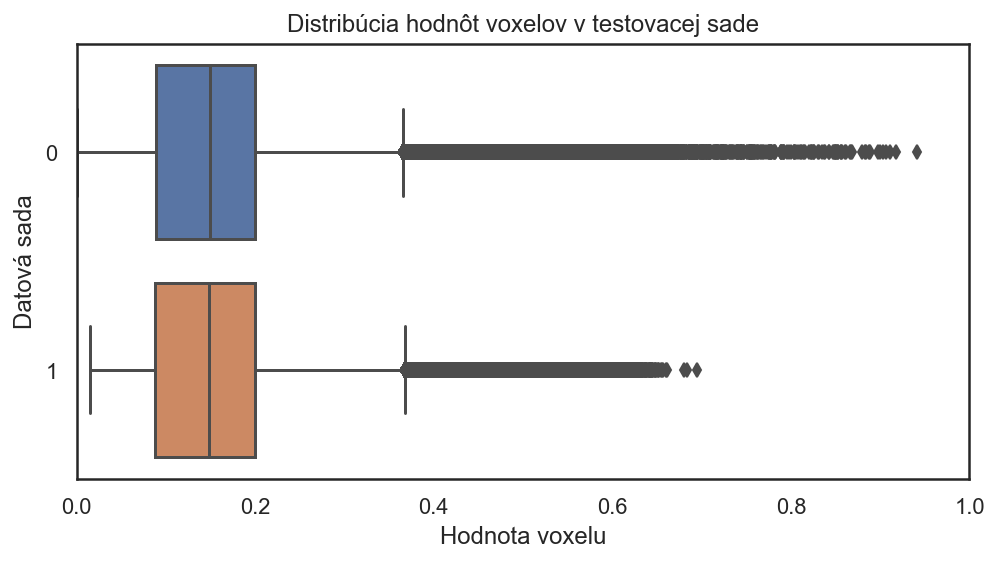
\includegraphics[width=11cm]{assets/images/test_dataset_voxel_distribution.png}
    \caption{Distribúcia hodnôt voxelov v trénovacej (0) a testovacej (1) sade. Testovacie dáta boli štandardizované (pred zmenšením) do intervalu $<0, 1>$ podľa maximálnych hodnôt v trénovacej sade.}
    \label{fig:test_dataset_voxel_distribution}
\end{figure}

\begin{table}[]
    \centering
    \begin{tabular}{l|l|l|}
        \cline{2-3}
                                                                    & \multicolumn{2}{c|}{Insertion} \\ \cline{2-3} 
                                                                    & Priemer        & Medián        \\ \hline
        \multicolumn{1}{|l|}{b1 =  0, b2 = 1, b2\_value = 0 (RISE)} & 0.43           & 0.37          \\ \hline
        \multicolumn{1}{|l|}{b1 =  0, b2 = 1, b2\_value = 1}        & \textbf{0.65}  & \textbf{0.67} \\ \hline
        \multicolumn{1}{|l|}{b1 =  0, b2 = 1, b2\_value = medián}     & 0.52           & 0.48          \\ \hline
        \multicolumn{1}{|l|}{b1 =  1, b2 = 0}                        & 0.53           & 0.47          \\ \hline
        \multicolumn{1}{|l|}{b1 =  1, b2 = 0.25, b2\_value = 0}     & 0.49           & 0.42          \\ \hline
        \multicolumn{1}{|l|}{b1 =  1, b2 = 0.50, b2\_value = 0}      & 0.44           & 0.37          \\ \hline
        \multicolumn{1}{|l|}{b1 =  1, b2 = 0.75, b2\_value = 0}     & 0.39           & 0.30          \\ \hline
    \end{tabular}
    \caption{\textbf{Porovnanie rôznych nastavení metódy RISEI.} Najlepšie výsledky dosiahla metóda bez použitia dokreslenia ale s prekrytím hodnotou jedna.}
    \label{tab:experiment_risei_various_configuration}
\end{table}

\begin{figure}[h!]
    \centering
    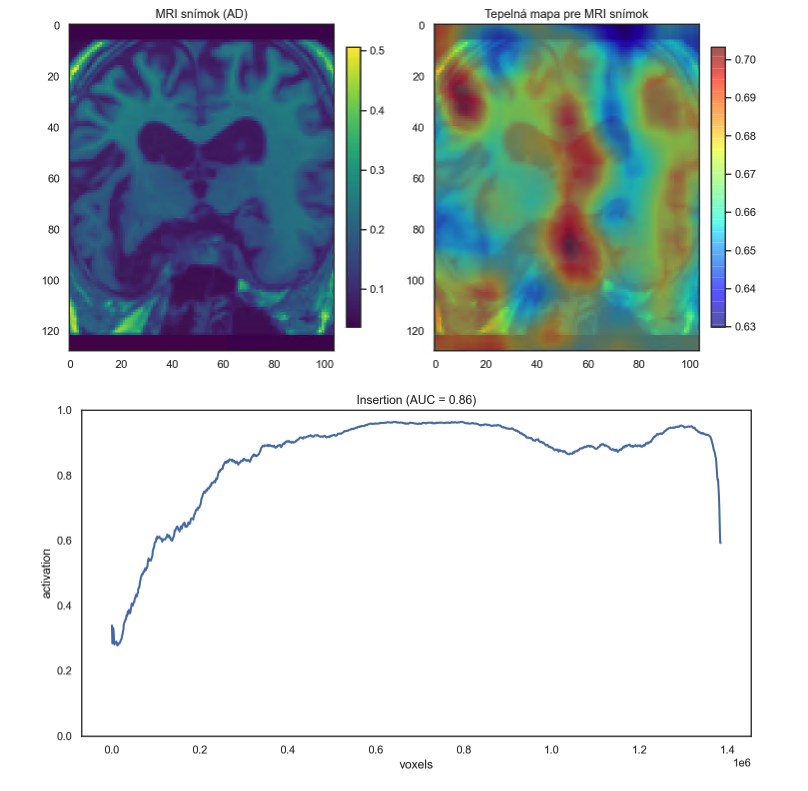
\includegraphics[width=14cm]{assets/images/heatmap_and_auc_example.png}
    \caption{Vytvorená tepelná mapa a graf zmeny aktivácie po pridávaní voxelov pre vybranú MRI snímku. Metrika AUC je pomerne vysoká, avšak je potrebné tepelnú mapu ešte vyhodnotiť z pohľadu segmentačných masiek. Tepelná mapa bola vytvorená s parametrami \textit{b1 = 1, b2 = 0} (RISEI s dokreslením).}
    \label{fig:heatmap_and_auc_example}
\end{figure}

Keďže sme neskôr natrénovali lepší model pre 3D CNN architektúru so senzitivitou 81\% a špecificitou 74\%, overlili sme ho v tomto experimente tiež, ale len na najlepšej zistenej kombinácii parametrov. Výsledok bola nižšia hodnota v metrike \textit{insertion} (priemer - 0.60, medián - 0.63). Vytvorené tepelné mapy medzi obomi modelmi boli veľmi podobné, no každý model ich vyhodnotil inak, tento problém sme načrtli v sekcii \ref{sec:experiment_rise_various_architectures}. Obrázok \ref{fig:3d_cnn_heatmap_cmp} zobrazuje takmer identicky vygenerované tepelné mapy, avšak lepší model, ktorý označil dané pozorovanie s vyššou istotou 
dosiahol nižšie skóre v metrike insertion. Tu sa črtá ďaľší problém metrík \textit{insertion} a \textit{deletion}, ak model vykazuje nižšiu mieru istoty pre pozorovanie - hodnota aktivácie, plocha pod krivkou (metrika AUC), ktorá k nej smeruje nemôže byť jedna. V našom prípade sú tieto aktivácie pomerne nízke (autori RISE uvádzali také príklady, kde aktivácie pre predikované triedy boli viac ako 0.9). Toto avšak nemusí byť nutne problém, keďže sa v snímke môžu nachádzať voxely, ktoré sú proti predikovanej triede, a teda mali nastavené teplo správne, a boli správne vložené až na konci vyhodnotenia. 

Ďaľším problémom týchto metrík môžu byť hodnoty voxelov, ktoré sú na miestach kde sme už zmazali/doposiaľ nepridali voxely, tie by mali byť neutrálne a nemali by hovoriť o žiadnej triede. My používame hodnotu nula (tá môže skôr hovoriť o AD pacientoch - chýbajúce tkanovo), avšak je tiež možné použiť opačný extrém, hodnotu jedna.

Aj kvôli zisteným problémom vyššie budeme tepelné mapy overovať voči segmentačným maskám aby sme získali lepšiu predstavu o správnosti tepelnej mapy. Aj napriek horšej metrike \textit{insertion} budeme ďalej používať lepšie natrénovaný model.

\begin{figure}[h!]
    \centering
    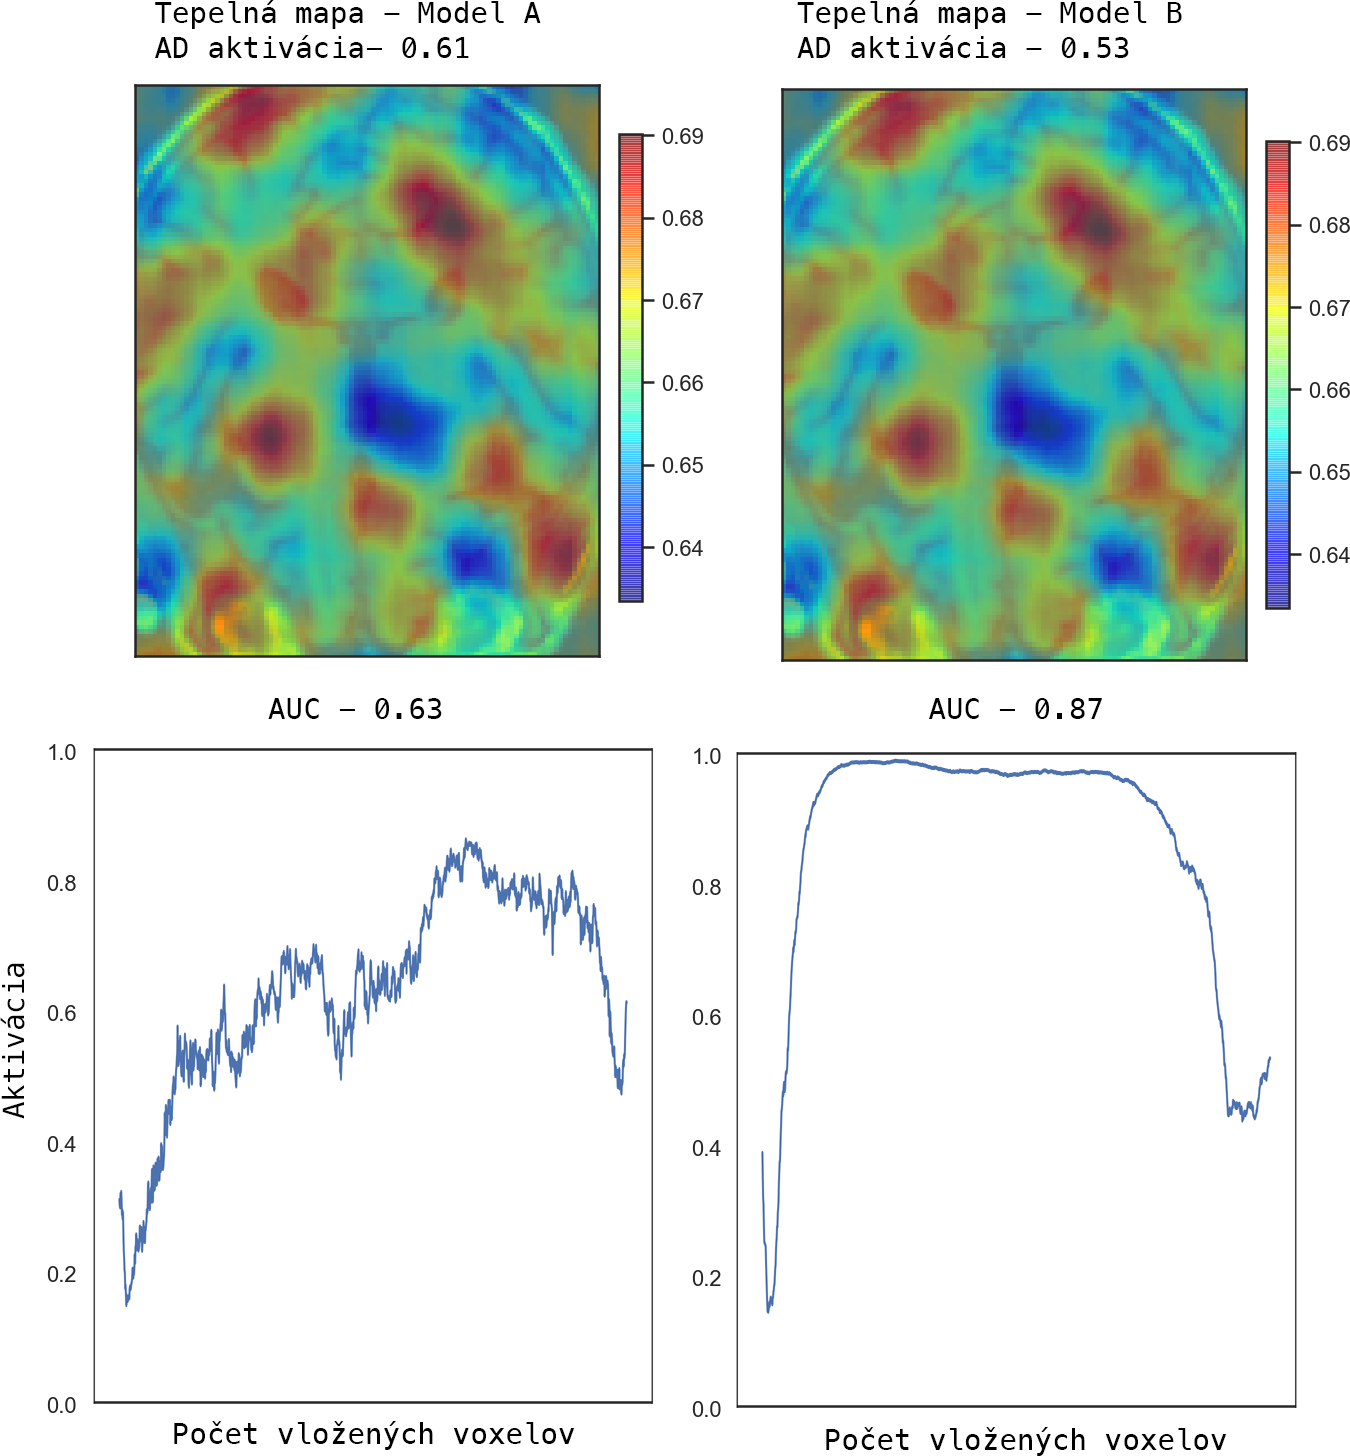
\includegraphics[width=14cm]{assets/images/3d_cnn_heatmap_cmp.png}
    \caption{Porovnanie tepelných máp vygenerovanými dvoma rôznymi modelmi. Model A) je model 3D CNN so senzitivitou 81\% a špecificitou 74\%. Model B) je model 3D CNN so senzitivitou 73\% a špecificitou 71\%. Oba modely vytvorili takmer identické tepelné mapy, avšak každý ich vyhodnotil inak. Kvalitatívne vyhodnotenie tepelnej mapy lepšie natrénovaného modelu dosiahlo horší výsledok.}
    \label{fig:3d_cnn_heatmap_cmp}
\end{figure}

\subsubsection{Nastavenie parametrov RISEI \label{sec:risei_parameters_experiment}}

Doposiaľ sme menili parametre \textit{b1}, \textit{b2} a \textit{b2\_value}, ktoré nastavujú hodnotu prekrytia v generovaných maskách. Okrem týchto parametrov má metóda RISEI ďaľšie parametre, ktoré nastavujú veľkosť prekrytia a počet generovaných masiek a významne ovplyvňujú výslednú tepelnú mapu. Vybrali sme 3 kombinácie parametrov, z predchádzajúcich experimentov, ktoré menia hodnotu prekrytia a to:

\begin{enumerate}[label=\Alph*]
    \item \textit{b1} = 0, \textit{b2} = 1 a \textit{b2\_value} = 0 (RISE),
    \item \textit{b1} = 0, \textit{b2} = 1 a \textit{b2\_value} = 1 (RISE s prekrytím hodnotou 1)
    \item \textit{b1} = 1, \textit{b2} = 0 (RISEI s dokreslením)
\end{enumerate}

čím sme zahrnuli pôvodnú metódu RISE, metódu RISEI s dokreslením a najlepšiu kombináciu parametrov. Tak ako sme uviedli v predchádzajúcom experimente, používame v tomto aj v ďaľších experiemntoch model 3D CNN so senzitivitou 81\% a špecificitou 74\%. Kvoli časovej náročnsoti týchto experimentov sme použili menšiu dátovu vzorku o veľkosti 10 pozorovaní (5 AD + 5 CN).

Aj tieto experimenty potvrdili, že metóda s prekryvom hodntou jedna dosahuje najlepšie výsledky. Ďalej sme zistili, že nastavením menšieho prekryvu (parameter \textit{p} má vyššiu hodnotu) sme v kombinácii s vyšším počtom masiek dosiahli lepšie výsledky, pričom od 256 masiek boli tieto hodnoty takmer rovnaké (Obr. \ref{fig:risei_parameters}). Od 2048 masiek boli dosiahnuté výsledky takmer rovnaké, toto môže súvisieť aj so stabilitou tepelných máp pri vyšších hodnotách (Sekcia \ref{sec:risei_stability}). Metódy RISEI a RISE s prekryvom nula dosiahli najlepšie výsledky s nízkym počtom masiek. Toto je prekvapivé, vzhľadom na to, že tepelné masky z nízkym počtom masiek niesú stabilné. Je preto možné, že sa jedná o chybu a náhodu, je to preto vhodné ďaľšie skúmanie.

\begin{sidewaysfigure}
    \centering
    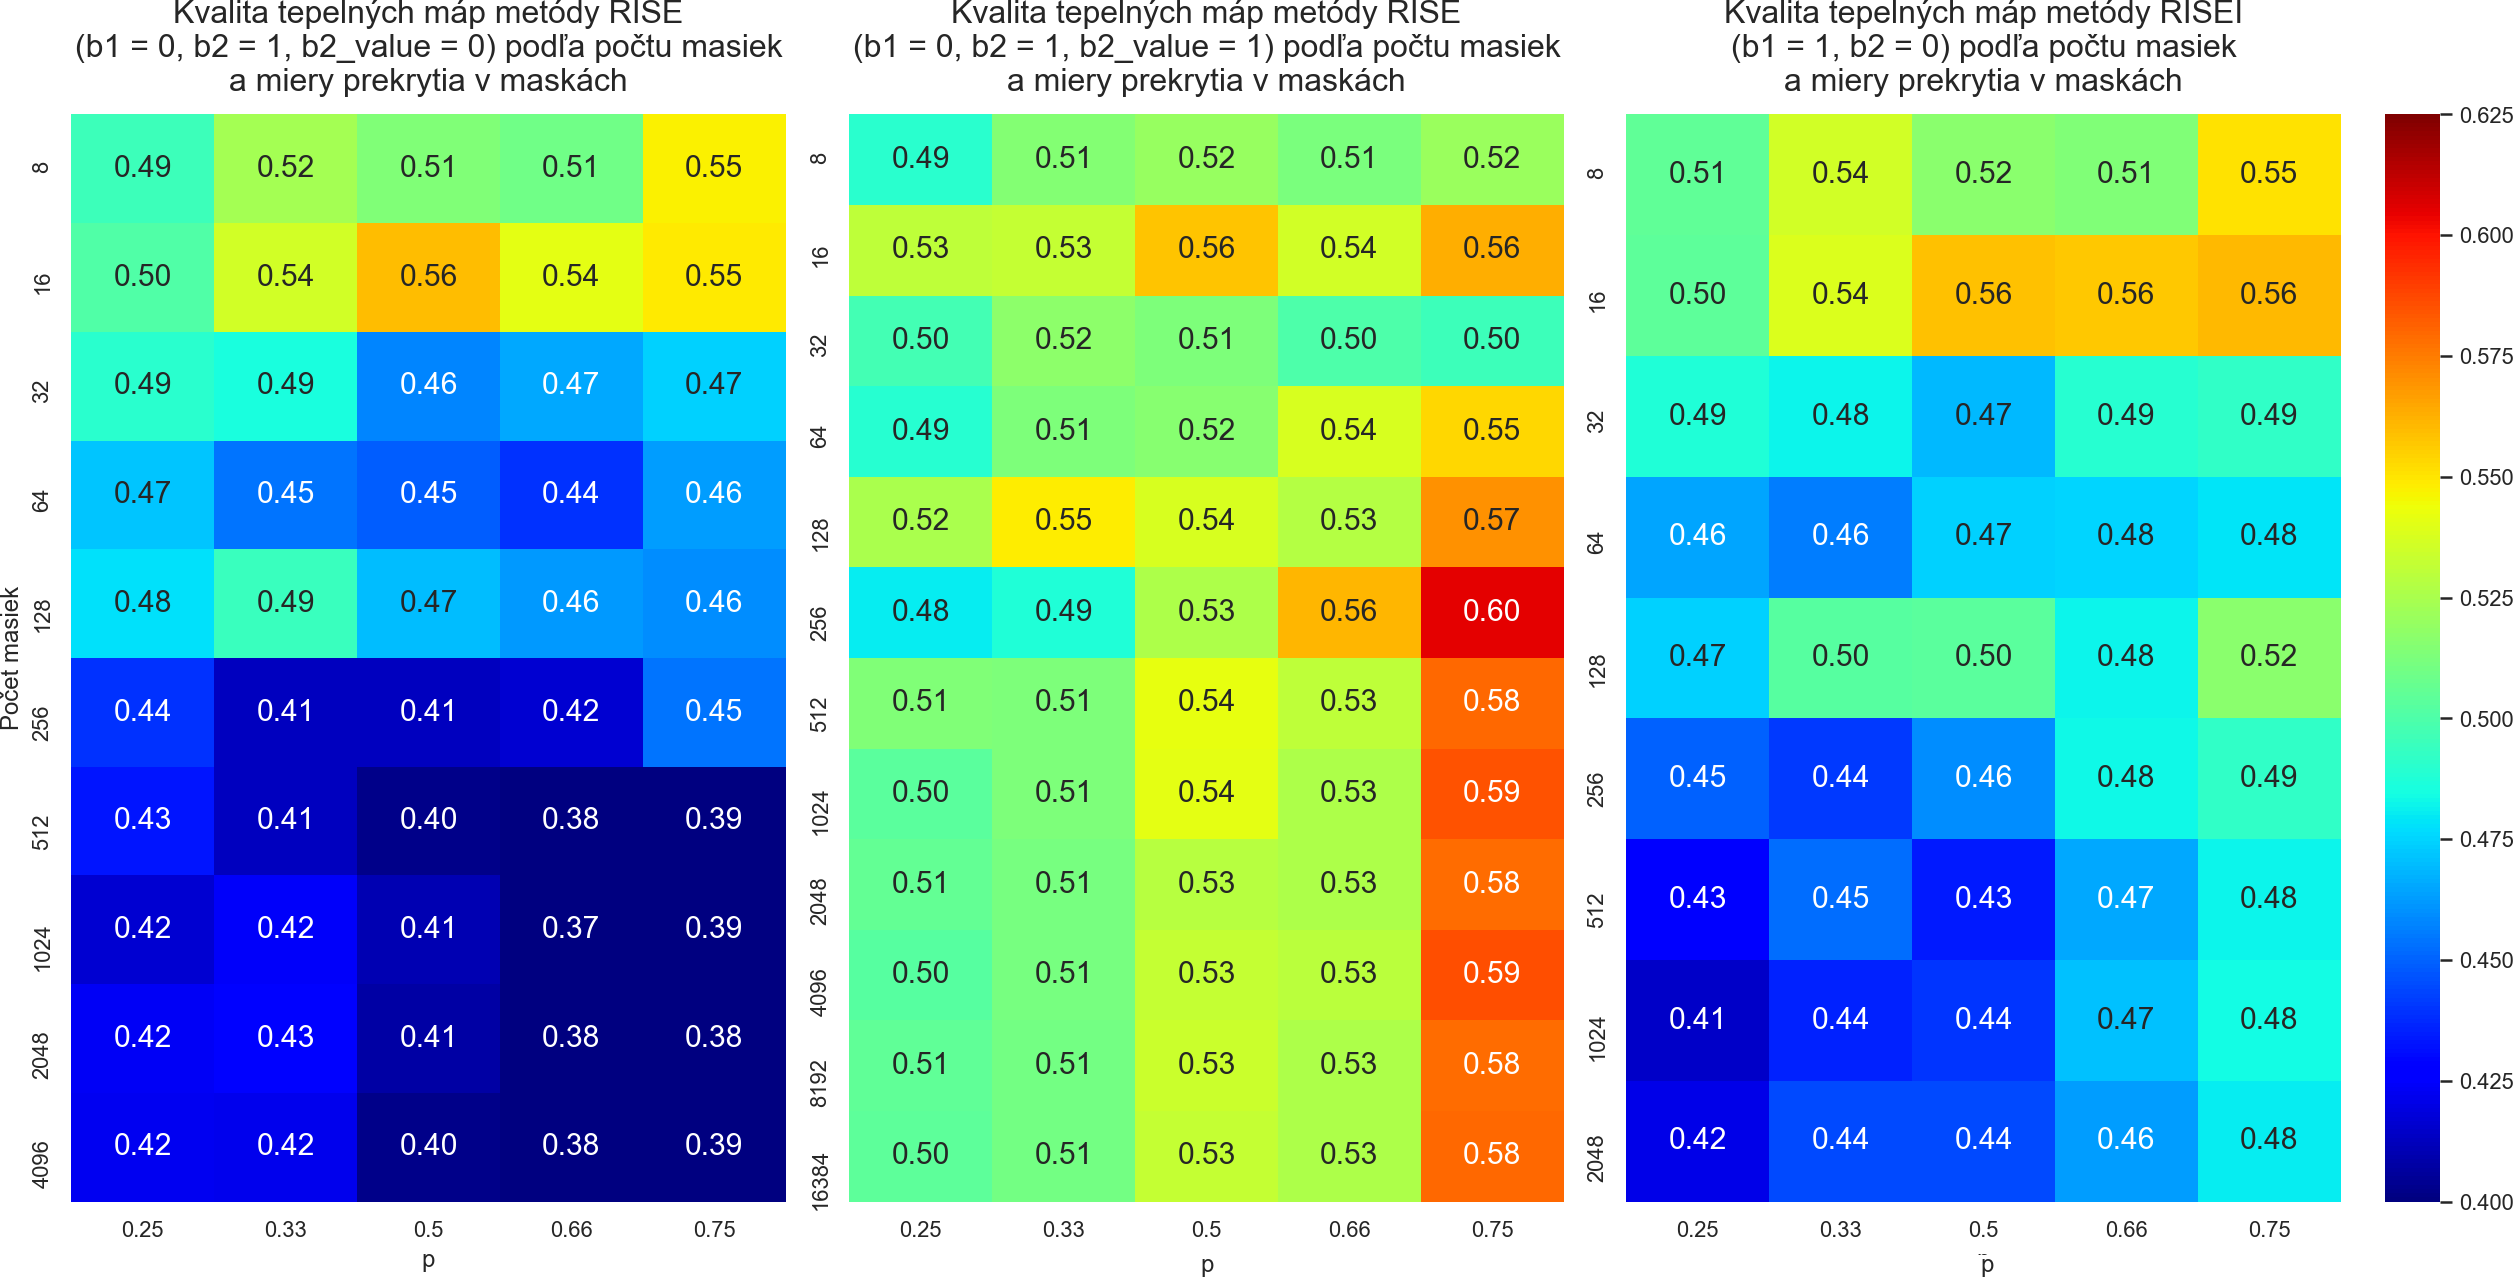
\includegraphics[width=20.6cm]{assets/images/risei_parameters.png}
    \caption{\textbf{Porovnanie kvality nastavených parametrov počtu masiek a veľkosti prekrytia (\textit{p}) na rôznych nastaveniach metódy RISEI.} Kvalitu sme merali ako $(insertion + (1 - deletion)) / 2$, z toho vyplýva, že čím vyššia hodnota, tým je vytvorená tepelná mapa kvalitnejšia. Keďže po 2048 generovaných maskách sa hodnoty výrazne nemenili (diagram v strede), tieto počty masiek sme vynechali v zvyšných experimentovh vynechali (digaramy vľavo a vpravo). Metóda RISEI s prekrytím 1 dosiahla najlepšie výsledky, zároveň vyššie hodnoty parametra \textit{p} sa ukázali ako lepšie.}
    \label{fig:risei_parameters}
\end{sidewaysfigure}

Parameter \textit{inpaint\_radius} sme za rozhodli netestovať, keďže z testov vyplynulo, že najvhodnejšie je prekrývať extrémnymi hodnotami, ktoré sú ojedinelé v dátach ($b2\_value = 1$). Zmena tohto parametra by znamenala, že by algoritmus použil iné okolité hodnoty - z nich by nevytvoril ojedinelé hodnotny.

\subsection{Porovnanie s existujúcimi metódami}

Všetky tri nastavenia metódy RISEI (vrátane metódy RISE) z predchádzajúceho experimentu (Sekcia \ref{sec:risei_parameters_experiment}) sme sa rozhodli porovnať s inými existujúcimi metódami. Na základe predchádzajúceho experimenty sme nastavili počet masiek na \textit{2048} a parameter \textit{p} na \textit{0.75}, keďže pri týchto parametroch sme dosiahli najlepšie výsledky a so zvoleným početom masiek sú tepelné mapy dostatočne stabilné (Sekcia \ref{sec:risei_stability}).

Z existujúcich metód sme vybrali metódy GradCAM, Guided Backprop a Guided GradCAM. Keďže sme sa rozhodli, že v našej práci venujeme čo najviac času experimentom a nie implementácii iných, už existujúcich metód, vybrali sme také metódy, ktoré nám ponúkala použitá knižnica \textit{captum} (preto sa neporovnávame s metódou LRP). V prípade metódy GradCAM a Guided GradCAM sme pri zväčšovaní konvolučnej vrsvy použili trilineárnu interpoláciu, keďže pracujeme s trojrozmernými dátami.

Zoznam porovnávaných metód je teda nasledovný:

\begin{enumerate}[label=\Alph*]
    \item RISE: \textit{b1} = 0, \textit{b2} = 1 a \textit{b2\_value} = 0,
    \item RISE s prekrytím hodnotou 1: \textit{b1} = 0, \textit{b2} = 1 a \textit{b2\_value} = 1,
    \item RISEI: \textit{b1} = 1, \textit{b2} = 0,
    \item GradCAM,
    \item Guided Backprop,
    \item Guided GradCAM,
    \item Guided RISE (s prekrytím hodnotou 1) - vypočítaný rovnako ako Guided GradCAM a to ako súčin tepelných máp po prvkoch medzi RISE a Guided Backprop.
\end{enumerate}

Ako testovaciu vzorku sme použili 40 pozorovaní (20 AD + 20 CN).

Vytvorené tepelné mapy sme porovnali aj oproti segmentačným maskám, v ktorých sme mali vyznačené nasledovné oblasti - šedá hmota, biela hmota, komory a hipokampus. V rámci týchto oblastí nás bude zaujímať koľko zachytili "tepla" z tepelných máp. Na základe ich veľkosti budeme následne počítať hustotu tepla ako $\frac{sucet\_tepla\_v\_oblasti}{pocet\_voxelov\_v\_ oblasti}$. Zároveň jednotlivé oblasti dáme do pomeru medzi sebou. 

\subsubsection{Metriky \label{sec:verification_experiments_metrics}}

Na vyhodnotenie tepelných máp pre každú snímku sme použili nasledovné metriky, pričom sme vychádzali z existujúcich prác popísaných v návrhu (\ref{sec:heat_maps_and_model_segmentation_masks}). 

Keďže tepelné mapy rôznych metód vyjadrujú teplo na rôznych škálach, tepelné mapy normalizujeme a preškálujeme ich do intervalu $<0, 1>$.

\begin{enumerate}[label=\Alph*]
    \item \textit{insertion x deletion} ($(insertion + (1 - deletion)) / 2$) - vyššia hodnota je lepšia,
    \item hustota tepla v jednotlivých častiach mozgu - šedá hmota, biela hmota, komory a hipokampus - vyššia hodnota je lepšia,
    \item pomer hustoty tepla mimo mozgu oproti hustote tepla v mozgu - nižšia hodnota je lepšia,
    \item pomer hustoty tepla zvyšnej časti snímky oproti významným častiam mozgu (biela hmota, komory a hipokampus) - nižšia hodnota je lepšia,
    \item pomer hustoty tepla mimo mozgu oproti významným častiam mozgu (biela hmota, komory a hipokampus) - nižšia hodnota je lepšia.
\end{enumerate}

\subsubsection{Výsledky \label{sec:verification_experiments_results}}

Najlepšie výsledky takmer vo všetkých metrikách dosiahla metóda Guided Backprop (Tabuľka \ref{tab:methods_evaluation}). 

Metriky \textit{B} nám dávajú predstavu o tom ako jednotlivé metódy rozdeľovali teplo a pomocou nich vieme koľko tepla bolo prodeleného mimo mozog. Všetky metódy rozdeľovali teplo pomerne rovnomerne medzi jednotlivé časti mozgu. U metódy GradCAM je na základe metriky \textit{C} vidieť, že CN pozorovaniam rozdelovala viac templa mimo mozog, toto je viditeľné aj na obrázku \ref{fig:method_evaluation_2}. Metrika \textit{C} je prvotným ukazovateľom ako dobre metóda funguje, najlepší výsledok v nej dosiahla metóda Guided Backprop, a to $0.808$. Táto hodnota je avšak pomerne vysoká, keďže hovorí, že hustota tepla mimo mozgu je až 80.8\% hustoty tepla v mozgu. Toto môže signalizovať zlý model. Podobne je tomu aj u metrík \textit{D} a \textit{E}. Metódy RISE nedosiahli dobré výsledky, najlepšie výsledky dosiahla metóda RISE s $b2\_value = 1$, pričom prekonala aj GradCAM.

Samotná metóda RISE dosiahla zo všetkych metód najhoršie výsledky, pričom ju prekonala aj metóda RISEI. Metóda RISE s prekrytím hodnotou jedna dosiahla porovnateľné výsledky s metódou GradCAM, pričom ju v niekoľkých metrikách (\textit{A}, \textit{C}) prekonala. Metóda Guided RISE nedokázala vylepšiť metódu Guided Backprop a bola s ňou v niekoľkých metrikách (\textit{C}, \textit{D}, \textit{E}) takmer totožná, v týchto metrikách dokonca prekonala metódu Guided GradCAM.

Zo sady pozorovaní sme vybrali sme dva snímky, jeden s najlepšou tepelnou mapou podľa metriky \textit{C} najlepšej metódy, druhú s najhoršou tepelnou mapou (Obr. \ref{fig:method_evaluation_1}, \ref{fig:method_evaluation_2}). Na základe vizualizácii nemôžeme tvrdiť, že by sa model rozhodoval na základe relevantných častí mozgu (Obr. \ref{fig:method_evaluation_2}). Metóda Guided Backprop zachytila pomerne veľké množstvo tepla na lebke mozgu, čo môže naznačovať, že máme chybný model.

\begin{small}
    \begin{table}
    \centering
    \begin{tabular}{|
    >{\columncolor[HTML]{C0C0C0}}l |r|r|r|r|r|r|r|}
    \hline
    \multicolumn{1}{|c|}{\cellcolor[HTML]{C0C0C0}\footnotesize{Metrika / Metóda}} &
        \multicolumn{1}{c|}{\cellcolor[HTML]{EFEFEF}\begin{tabular}[c]{@{}c@{}}\small{Grad-}\\ \small{CAM}\end{tabular}} &
        \multicolumn{1}{c|}{\cellcolor[HTML]{EFEFEF}\begin{tabular}[c]{@{}c@{}}\small{Guided}\\ \small{Back-}\\\small{prop}\end{tabular}} &
        \multicolumn{1}{c|}{\cellcolor[HTML]{EFEFEF}\begin{tabular}[c]{@{}c@{}}\small{Guided}\\ \small{Grad-}\\ \small{CAM}\end{tabular}} &
        \multicolumn{1}{c|}{\cellcolor[HTML]{EFEFEF}\begin{tabular}[c]{@{}c@{}}\small{Guided}\\ \small{RISE}\\ \small{(b2\_}\\ \small{value}\\ \small{= 0})\end{tabular}} &
        \multicolumn{1}{c|}{\cellcolor[HTML]{EFEFEF}\begin{tabular}[c]{@{}c@{}}\small{RISE}\\ \small{(b2\_}\\ \small{value}\\ \small{= 0)}\end{tabular}} &
        \multicolumn{1}{c|}{\cellcolor[HTML]{EFEFEF}\begin{tabular}[c]{@{}c@{}}\small{RISE}\\ \small{(b2\_}\\ \small{value}\\ \small{= 1)}\end{tabular}} &
        \multicolumn{1}{c|}{\cellcolor[HTML]{EFEFEF}\footnotesize{RISEI}} \\ \hline
    A (AD + CN)                                                         & 0.572 & \textbf{0.678} & 0.673 & 0.547 & 0.401 & 0.610 & 0.443 \\ \hline
    A (AD)                                                              & 0.606 & 0.803 & \textbf{0.810} & 0.552 & 0.372 & 0.550 & 0.423 \\ \hline
    A (CN)                                                              & 0.541 & 0.564 & 0.538 & 0.473 & 0.426 & \textbf{0.638} & 0.462 \\ \hline
    \begin{tabular}[c]{@{}l@{}}B - biela hmota\\ (AD + CN)\end{tabular} & 0.466 & 0.607 & 0.507 & 0.606 & 0.497 & 0.512 & 0.498 \\ \hline
    \begin{tabular}[c]{@{}l@{}}B - hipokampus\\ (AD + CN)\end{tabular}  & 0.400 & 0.559 & 0.500 & 0.556 & 0.491 & 0.435 & 0.501 \\ \hline
    \begin{tabular}[c]{@{}l@{}}B - komory\\ (AD + CN)\end{tabular}      & 0.417 & 0.333 & 0.491 & 0.331 & 0.494 & 0.537 & 0.484 \\ \hline
    \begin{tabular}[c]{@{}l@{}}B - nie mozog \\ AD + CN)\end{tabular}   & 0.503 & 0.464 & 0.498 & 0.464 & 0.502 & 0.494 & 0.500 \\ \hline
    \begin{tabular}[c]{@{}l@{}}B - šedá hmota\\ (AD + CN)\end{tabular}  & 0.452 & 0.572 & 0.504 & 0.571 & 0.499 & 0.504 & 0.503 \\ \hline
    C (AD + CN)                                                         & 1.108 & \textbf{0.808} & 0.986 & 0.809 & 1.014 & 0.970 & 1.002 \\ \hline
    C (AD)                                                              & 0.854 & \textbf{0.810} & 0.942 & \textbf{0.810} & 0.985 & 0.996 & 1.004 \\ \hline
    C (CN)                                                              & 1.234 & \textbf{0.802} & 0.999 & 0.803 & 1.015 & 0.968 & 0.999 \\ \hline
    D (AD + CN)                                                         & 1.118 & \textbf{0.875} & 0.991 & \textbf{0.875} & 1.000 & 0.989 & 0.999 \\ \hline
    D (AD)                                                              & 0.948 & \textbf{0.882} & 0.970 & \textbf{0.882} & 0.991 & 1.005 & 0.990 \\ \hline
    D (CN)                                                              & 1.171 & \textbf{0.868} & 0.998 & 0.869 & 1.004 & 0.983 & 1.005 \\ \hline
    E (AD + CN)                                                         & 1.130 & \textbf{0.836} & 0.989 & 0.837 & 1.004 & 0.982 & 0.995 \\ \hline
    E (AD)                                                              & 0.910 & \textbf{0.840} & 0.957 & 0.841 & 0.984 & 1.002 & 0.993 \\ \hline
    E (CN)                                                              & 1.206 & \textbf{0.828} & 0.998 & 0.830 & 1.006 & 0.975 & 1.002 \\ \hline
    \end{tabular}
    \caption{\textbf{Porovnanie kvality a správnosti tepelných máp RISEI oproti iným existujúcim metódam.}
    Hodnoty jednotlivých metrík sú strednými hodnotami metrik pre jednotlivé pozorovania v testovacej sade. Popis metrík sa nachadza v sekcii \ref{sec:verification_experiments_metrics}}
    \label{tab:methods_evaluation}
    \end{table}
\end{small}

\begin{figure}[h!]
    \centering
    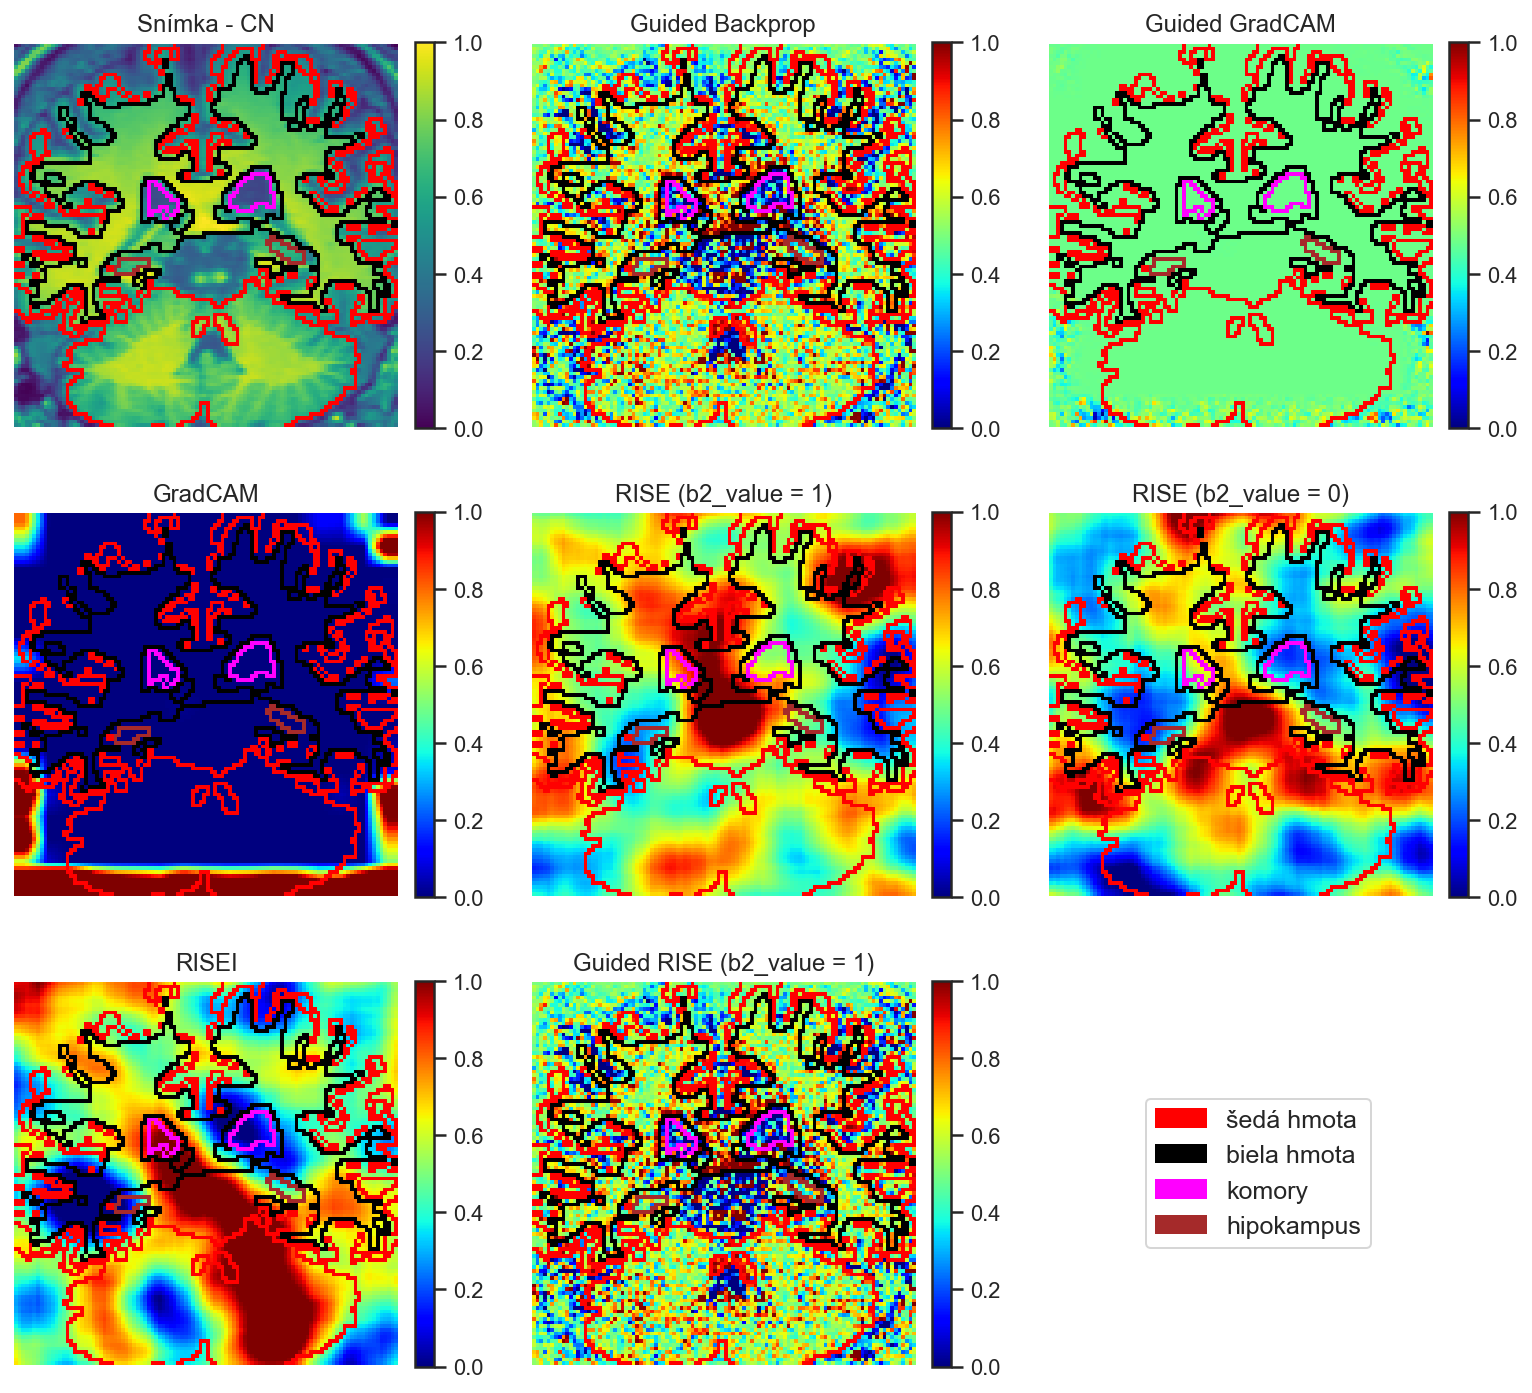
\includegraphics[width=13cm]{assets/images/method_evaluation_2.png}
    \caption{Porovnanie tepelných máp vytvorených porovnávaními metódami. Vybrali sme snímku s najlepšiou tepelnú mapu pre metódu Guided Backprop podľa metriky \textit{C = 0.781}. Tak ako aj na obrázku \ref{fig:method_evaluation_1}, aj tu si môžeme všimnúť výrazné rozdiely medzi jednotlivými metódami. Metóda GradCAM pridelila veľmi málo tepla do mozgu a veľmi málo tepla na krajoch snímky.}
    \label{fig:method_evaluation_2}   
\end{figure}

\begin{figure}[h!]
    \centering
    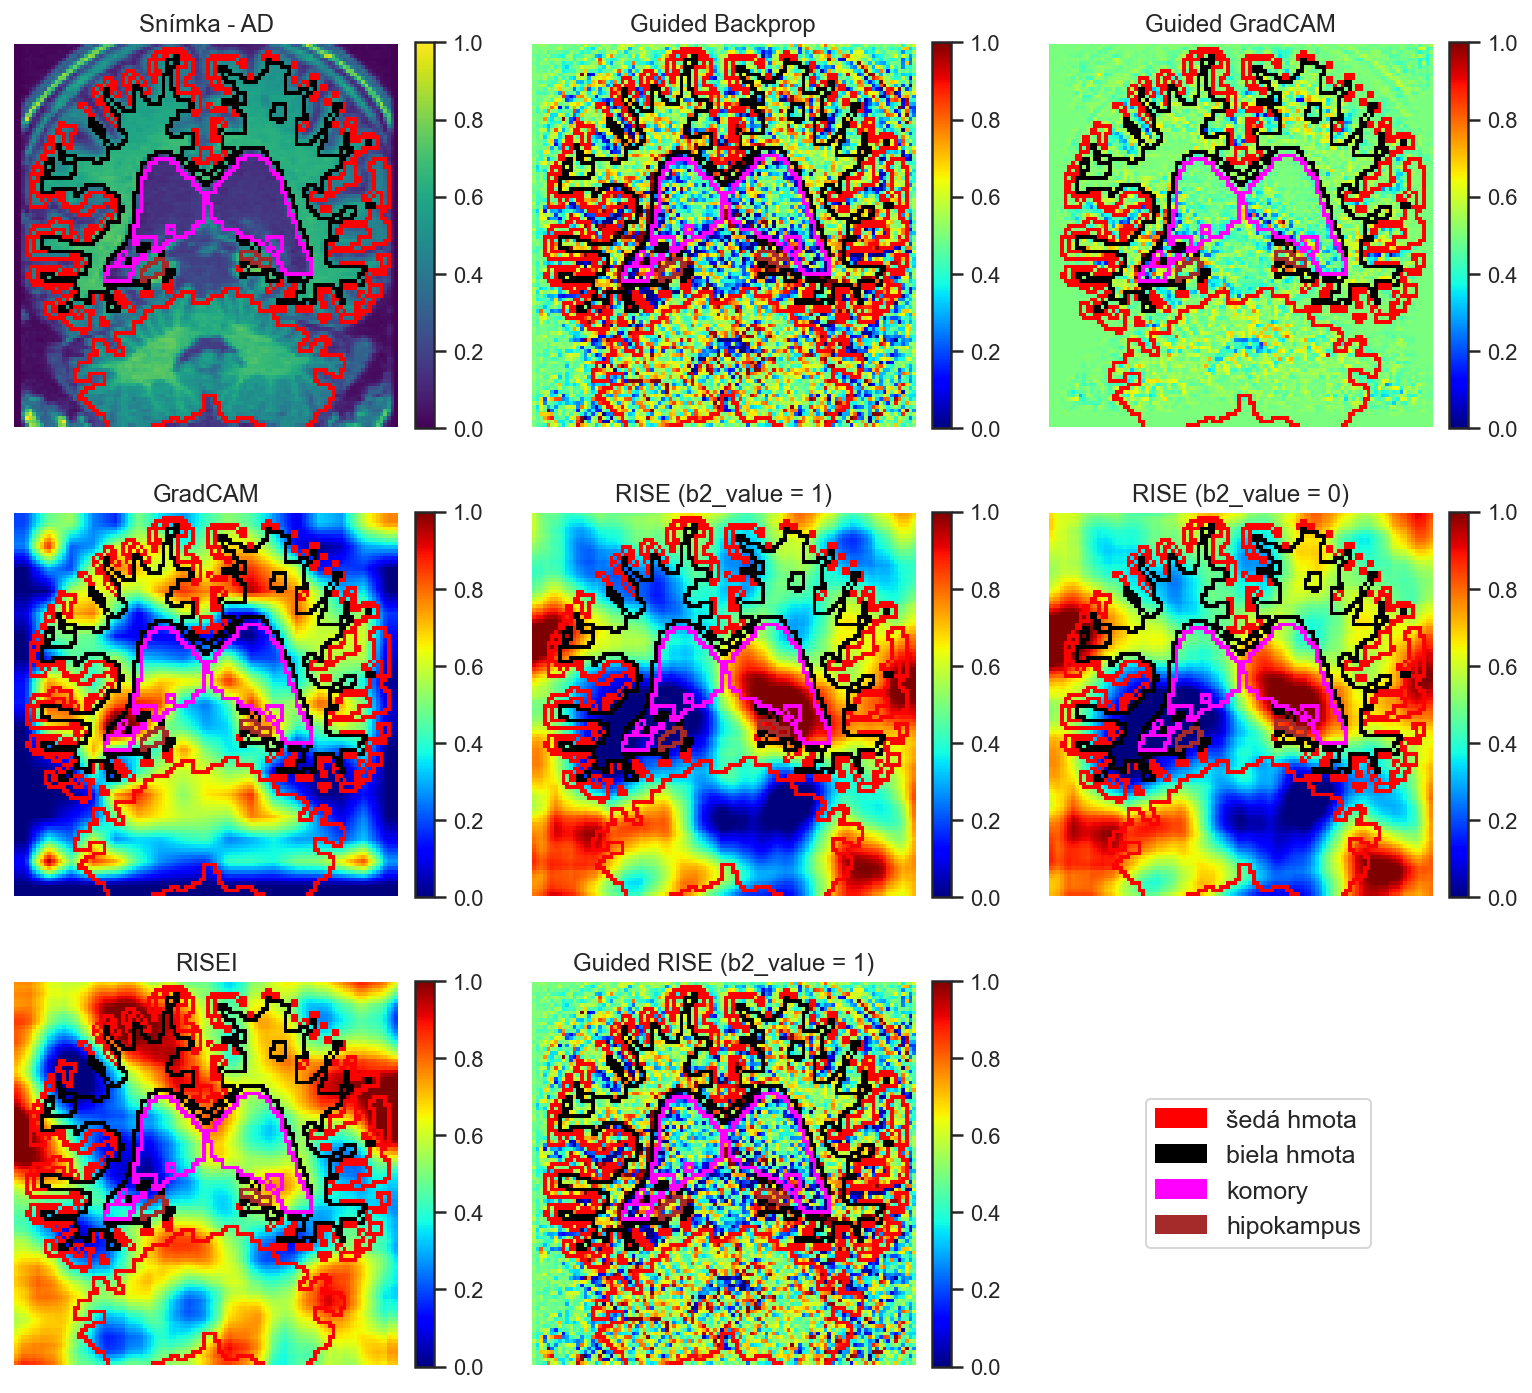
\includegraphics[width=14.5cm]{assets/images/method_evaluation_1.png}
    \caption{\small{Porovnanie tepelných máp vytvorených porovnávaními metódami. Vybrali sme snímku s najlepšiou tepelnú mapu pre metódu Guided Backprop podľa metriky \textit{C = 0.839}. Môžeme si všimnúť výrazné rozdiely medzi jednotlivými metódami. Teplo z metódy Guided Backprop, ktoré sa nachádza mimo mozgu, lemuje časť lebky, v ľavej a aj v pravej časti snímky. Metóda GradCAM oproti metódam RISE rozdelila pomerne veľa tepla v rámci mozgu.}}
    \label{fig:method_evaluation_1}
\end{figure}

% TODO: compare the best and the worst heatmaps 

\section{Zhrnutie}

Metódu RISE sme otestovali na niekoľkých architektúrach neurónových sietí pričom architektúrou, ktorú sme vyhodnotili ako navhodnejšiu pre ďaľšie experimenty sme použili v ďaľších experimentoch. Nevyhodnocovali sme, ktorý model je najlepší, pretože použité metriky \textit{insertion} a \textit{deletion} nie sú na takútou úlohu vhodné.

Podarilo sa nám vyhodnotiť stabilitu vytváraných tepelných máp. Z výsledkov sme usúdili, že so stúpajúcim počtom generovaných masiek stúpa stabilita vytvárania tepelných máp pričim chyba po určitom počte je už zanedbateľná.

Vyhodnotili sme rôzne hodnoty prekrytia pre metódu RISEI. Následne sme hľadali optimálny počet masiek a mieru prekrytia.

Metódu RISEI (a jej rôzne nastavenia na základe doterajších experimentov) sa nám podarilo porovnať s niekoľkými existujúcimi metódami. Pričom v sledovaných metrikách sme dosiahli horšie výsledky ako metóda Guided Backprop, ktorá vo väčšine metrík dominovala.

Dosiahnuté výsledky naznačujú, že máme model, ktorý sa nerozhoduje na základe relevantných častí mozgu - rozhoduje napr. aj na základe lebky. Toto má vo veľkej miere vyplyv na kvalitu tepelných máp metódy RISE, keďže vytvára tepelné mapy z veľkého počtu predikcií k zamaskovaným snímkam. Ďaľšie experimenty by bolo vhodné realizovať na modeli s lepšou úspešnosťou a na pozorovaniach s odstránenou lebkou zo snímiek v predspracovaní.


% Zistili sme, že metóda RISE s dokresľovaním dosahuje lepšie výsledky ako pôvodná metóda ktorá zakrývala minimálnou hodnotou. Pokial ale minimálnu hodnotu nahradíme maximálnou, dosiahneme lepšie výsledky ako s dokreslovaním, ktoré dosahuje podobné vśyeldky ako zakrývaním mediánom. Avšak, vyhodnocovali sme zatiaľ len pomerne malej vzorke a nebrali sme do úvahy početnosť tried (AD a CN) v tejto vzorke čo je nedostatkom našich experimentov (v ďaľších experimentoch by mali byť tieto triedy vyvážené). Zároveň na dátach z tejto vzorky nemali testované modely 100\%-nú úspešnosť.

% Na generovanie tepelných máp sme použili 1000 masiek (keďže autori metódy RISE v experimentoch použili podobný počet), avšak my máme iný typ dát (3D volumetrické dáta), preto je vhodné vyskúšať rôzne počty a nájsť vhodný počet pre náš problém.

% Keďže sú masky pri generovaní tepelných máp náhodné, je možné, že pre jeden MRI snímok metóda vygeneruje rôzne tepelné masky. V ďaľších experimentoch by sme mali vyhodnocovať aj konzistenciu tepelných máp - tj. ako veľmi sa líšia medzi rôznymi použitiami metódy na tom istom snímku. Predpokladáme, že väčší počet použitých másk bude viesť ku konzistentnejším tepelným mapám. Takýmto meraním môžeme dospieť k optimálnemu počtu masiek, ktorý je potrebný na generovanie tepelnej mapy.

% Taktiež je potrebné vyhodnotiť správnosť tepelných máp vzhľadom na segmentačné masky, tak ako sme uviedli v návrhu riešenia (Sekcia \ref{sec:heat_maps_and_model_segmentation_masks}). Ďalej je potrebné porovnať navrhovanú metódy s inými existujúcimi metódami, napr. LRP alebo analýza senzitivity.


% TODO: we need to compare our method with other methods like LRP or other oclussion methods
% TODO: evaluate the consistency of heatmaps, the method several times for the same image and find out if heatmaps are consistent - this way we can find also optimal number of masks
% TODO: compare with segmentation masks, if more heat is in important areas
